\documentclass[12pt]{article}

\usepackage[utf8]{inputenc}
\usepackage{graphicx,url,caption,titlesec,geometry}
\usepackage{times}
\geometry{a4paper,top=3.5cm,left=3cm,right=3cm,bottom=2.5cm}
\parindent 1.27cm
\parskip   6pt
\newenvironment{resumo}{\begin{quote}\textbf{Resumo.}\itshape}{\end{quote}}

\sloppy

\title{Dilema do Prisioneiro em Autômato Unidimensional: reprodução e resultados}

\author{Grupo: Helcio Duarte, Pedro Henrique Guedes, Rafael Vieira}
\begin{document}

\maketitle

\begin{abstract}
Apresentamos a reprodução computacional do experimento de Pereira et al. (2008)
que investiga o Dilema do Prisioneiro espacial em autômatos unidimensionais.
Implementamos a dinâmica proposta, realizamos varredura no parâmetro "tentação" $T$
e calculamos a proporção assintótica média de cooperadores $\rho_{\infty}(T)$.
As figuras e dados gerados são apresentados e discutidos.
\end{abstract}

\begin{resumo}
Reproduzimos o experimento de Pereira et al. (2008) para o Dilema do Prisioneiro em autômato
unidimensional. Foram realizadas simulações com varredura no parâmetro $T$ e ensembles para
estimar $\rho_{\infty}$. Relatamos metodologia, resultados e discussão comparativa.
\end{resumo}

\section{Introdução}
O Dilema do Prisioneiro espacial é um paradigma para estudar a emergência de cooperação.
Seguindo Pereira et al. (2008), implementamos jogadores em uma rede unidimensional onde
cada jogador interage com $z$ vizinhos e atualiza sua estratégia copiando o vizinho com maior
payoff caso este supere seu próprio payoff. Nosso objetivo foi reproduzir a curva $\rho_{\infty}(T)$
e visualizar padrões espaço-temporais (triangles, fingers, gliders) reportados no artigo.

\section{Metodologia}
  \textbf{Implementação:} Código em Python com vetorização em \texttt{numpy}; a biblioteca usa
rolamentos (\texttt{np.roll}) para somar estados dos vizinhos e operações vetoriais para escolher
os vencedores. A rotina de ensembles foi paralelizada com \texttt{multiprocessing.Pool} para usar
vários workers e permitir ensembles grandes de forma prática.

\subsection{Modelagem formal}
Cada jogador $i$ possui estado $\theta_i\in\{0,1\}$ (0=desertor, 1=cooperador). O ganho obtido
na interação entre $i$ e $j$ é dado por (Eq. (1) do artigo):
\[
g_{\theta_i,\theta_j} = \theta_i\theta_j + T(1-\theta_i\theta_j)\theta_j
\]
O payoff total de $i$ é a soma sobre os $z$ vizinhos (incluindo autointeração quando aplicável):
\[
P_i = \sum_{j\in V_i} g_{\theta_i,\theta_j}.
\]
Observando que, se $c$ é o número de cooperadores na vizinhança de $i$, o payoff pode ser escrito
compactamente como (Eq. (3) do artigo):
\[
P_i^{(c)}(\theta_i) = [T - (T-1)\theta_i]\, c.
\]
O procedimento de atualização é síncrono: para cada jogador, comparamos seu payoff com o máximo
dos payoffs dos vizinhos; se existir vizinho com payoff estritamente maior, o jogador copia a estratégia
desse vizinho no próximo passo de tempo.

\subsection{Parâmetros do experimento}
\begin{itemize}
  \item Tamanho da rede: $L=1000$;
  \item Proporção inicial de cooperadores: $\rho_0=0.7$;
  \item Número de rodadas por simulação: 500;
  \item Vizinhança: $z=7$ (simétrica com autointeração quando aplicável);
  \item Varredura: $T\in[1.0,2.0]$ com passo $\Delta T=0.05$;
  \item Ensemble por valor de $T$: 100 réplicas (executado usando paralelização em 8 workers);
\end{itemize}

As simulações foram executadas com sementes pseudoaleatórias variando por réplica; os parâmetros e
metadados de cada execução foram gravados localmente.

\section{Resultados}
Geramos a curva $\rho_{\infty}(T)$ calculando a média e o desvio padrão das réplicas para cada valor
de $T$. A Tabela~\ref{tab:rho} resume os resultados. O arquivo CSV completo foi salvo em
\verb|../artigo-deps/rho_infty_vs_T.csv| e o gráfico em
\verb|impl/exp_full/rho_infty_vs_T.png|.

\begin{table}[ht]
\centering
\caption{Proporção assintótica média de cooperadores $\rho_{\infty}$ como função de $T$ (varredura com 100 réplicas).}
\label{tab:rho}
\begin{tabular}{c c c}
\hline
T & $\rho_{\infty}$ (média) & desvio padrão \\
\hline
1.00 & 0.96656 & 0.00440 \\
1.05 & 0.98669 & 0.00341 \\
1.10 & 0.98605 & 0.00343 \\
1.15 & 0.98617 & 0.00375 \\
1.20 & 0.91976 & 0.01887 \\
1.25 & 0.93801 & 0.01761 \\
1.30 & 0.94221 & 0.01819 \\
1.35 & 0.94468 & 0.01513 \\
1.40 & 0.94514 & 0.01521 \\
1.45 & 0.97194 & 0.01109 \\
1.50 & 0.98070 & 0.00679 \\
1.55 & 0.98257 & 0.00584 \\
1.60 & 0.98359 & 0.00694 \\
1.65 & 0.98326 & 0.00653 \\
1.70 & 0.96729 & 0.01164 \\
1.75 & 0.96872 & 0.01450 \\
1.80 & 0.96125 & 0.09761 \\
1.85 & 0.97343 & 0.01184 \\
1.90 & 0.97394 & 0.01231 \\
1.95 & 0.96357 & 0.09763 \\
2.00 & 0.02968 & 0.01989 \\
\hline
\end{tabular}
\end{table}

O gráfico de $\rho_{\infty}(T)$ (Figura~\ref{fig:rhoT}) destaca uma queda abrupta em $T=2.0$,
enquanto em grande parte do intervalo a cooperação persiste com alta fração de cooperadores.

\begin{figure}[ht]
\centering
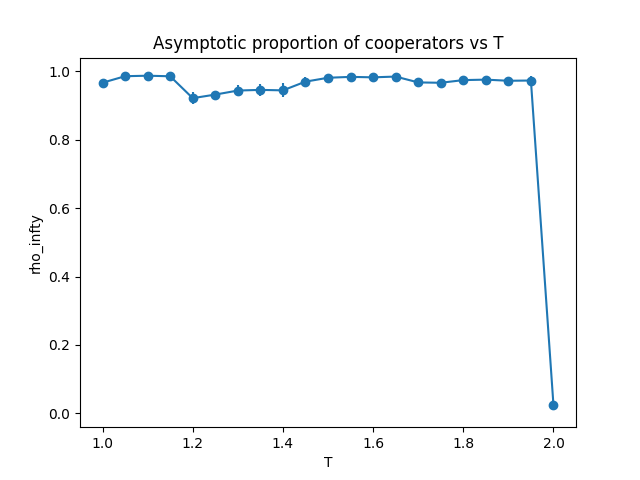
\includegraphics[width=.7\textwidth]{../artigo-deps/rho_infty_vs_T.png}
\caption{Curva $\rho_{\infty}$ vs $T$ (média com barras de erro = desvio padrão).}
\label{fig:rhoT}
\end{figure}

Para ilustrar padrões espaço-temporais, geramos uma simulação representativa em $T=1.20$.
Figura~\ref{fig:spacetime} mostra o mapa espaço-temporal (eixo X = jogador, eixo Y = tempo), onde
azul = cooperador estável, vermelho = desertor estável, verde = virou cooperador, amarelo = virou desertor.

\begin{figure}[ht]
\centering
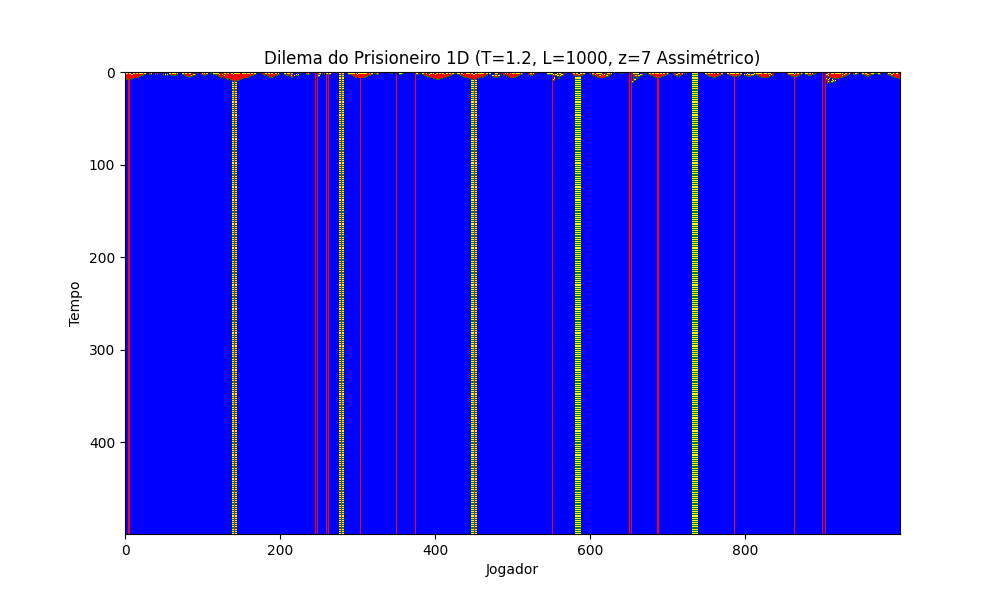
\includegraphics[width=.7\textwidth]{../artigo-deps/space_time_T1.200.png}
\caption{Mapa espaço-temporal representativo para $T=1.20$ (L=1000, rodadas=500).}
\label{fig:spacetime}
\end{figure}

\section{Discussão}
Os resultados mostram que a cooperação é robusta para grande parte de $T$ na configuração estudada,
em acordo qualitativo com Pereira et al. (2008). Observou-se uma queda drástica em $T\approx2.0$,
coerente com a expectativa teórica de transição quando a tentação é muito alta.

\subsection{Ambiente de execução}
As simulações foram executadas no ambiente WSL2 do autor com as seguintes especificações:
\begin{itemize}
  \item Kernel/OS: Linux rafael 6.6.87.2-microsoft-standard-WSL2 (x86\_64);
  \item CPU: AMD Ryzen 5 5500, 6 cores / 12 threads (relatados como 12 CPUs virtuais);
  \item Memória: 3.8 GiB total (aprox. 1.9 GiB disponível durante as execuções);
  \item Python: Python 3.12.3 (ambiente virtual utilizado para dependências: numpy, matplotlib);
  \item Parâmetros de execução: varredura com 100 réplicas por T, 8 workers paralelos.
\end{itemize}

Esses detalhes são relevantes para reprodutibilidade e tempo de execução dos ensembles.

Padrões espaço-temporais observados (triangles, gliders e fingers) aparecem nas figuras e podem ser
analisados quantitativamente em trabalhos posteriores. Diferenças quantitativas em $\rho_{\infty}(T)$
podem derivar de (i) número finito de réplicas usado aqui (100), (ii) sutilidades na definição exata de
vizinhança e autointeração, e (iii) parâmetros iniciais.

\section{Conclusão}
Implementamos e reproduzimos a dinâmica do Dilema do Prisioneiro em autômatos unidimensionais.
Geramos a curva $\rho_{\infty}(T)$ e mapas espaço-temporais representativos. Próximos passos incluem
ampliar o ensemble, paralelizar execuções e preparar os resultados finais no template SBC para
submissão.

\begin{thebibliography}{9}
\bibitem{pereira2008}
M. A. Pereira, A. S. Martinez, A. L. Espindola,
"Prisoner's Dilemma in One-dimensional Cellular Automata: Visualization of Evolutionary Patterns",
Int. J. Mod. Phys. C, 19, 187--201 (2008).

\bibitem{nowak1992}
M. A. Nowak and R. M. May,
"Evolutionary Games and Spatial Chaos",
Nature 359, 826--829 (1992).
\end{thebibliography}

\end{document}
